To manage our software we are using \textit{Rust},
as the main language of development, due to its high expressibility and low level management.
We utilise methods such as Test-Driven-Developmen with the help of \texttt{Proptest},
for property testing and kanban boards to accurately track our progress as seen
in the figure \ref{fig:management:tooling}. Lastly we are making use of 
\textit{Bevy} which is a game engine that use the Entitiy-Component-System
for render interactinos between entities as seen in \ref{fig:soft:ecs-workflow}.


\begin{figure}[h!]
    \centering
    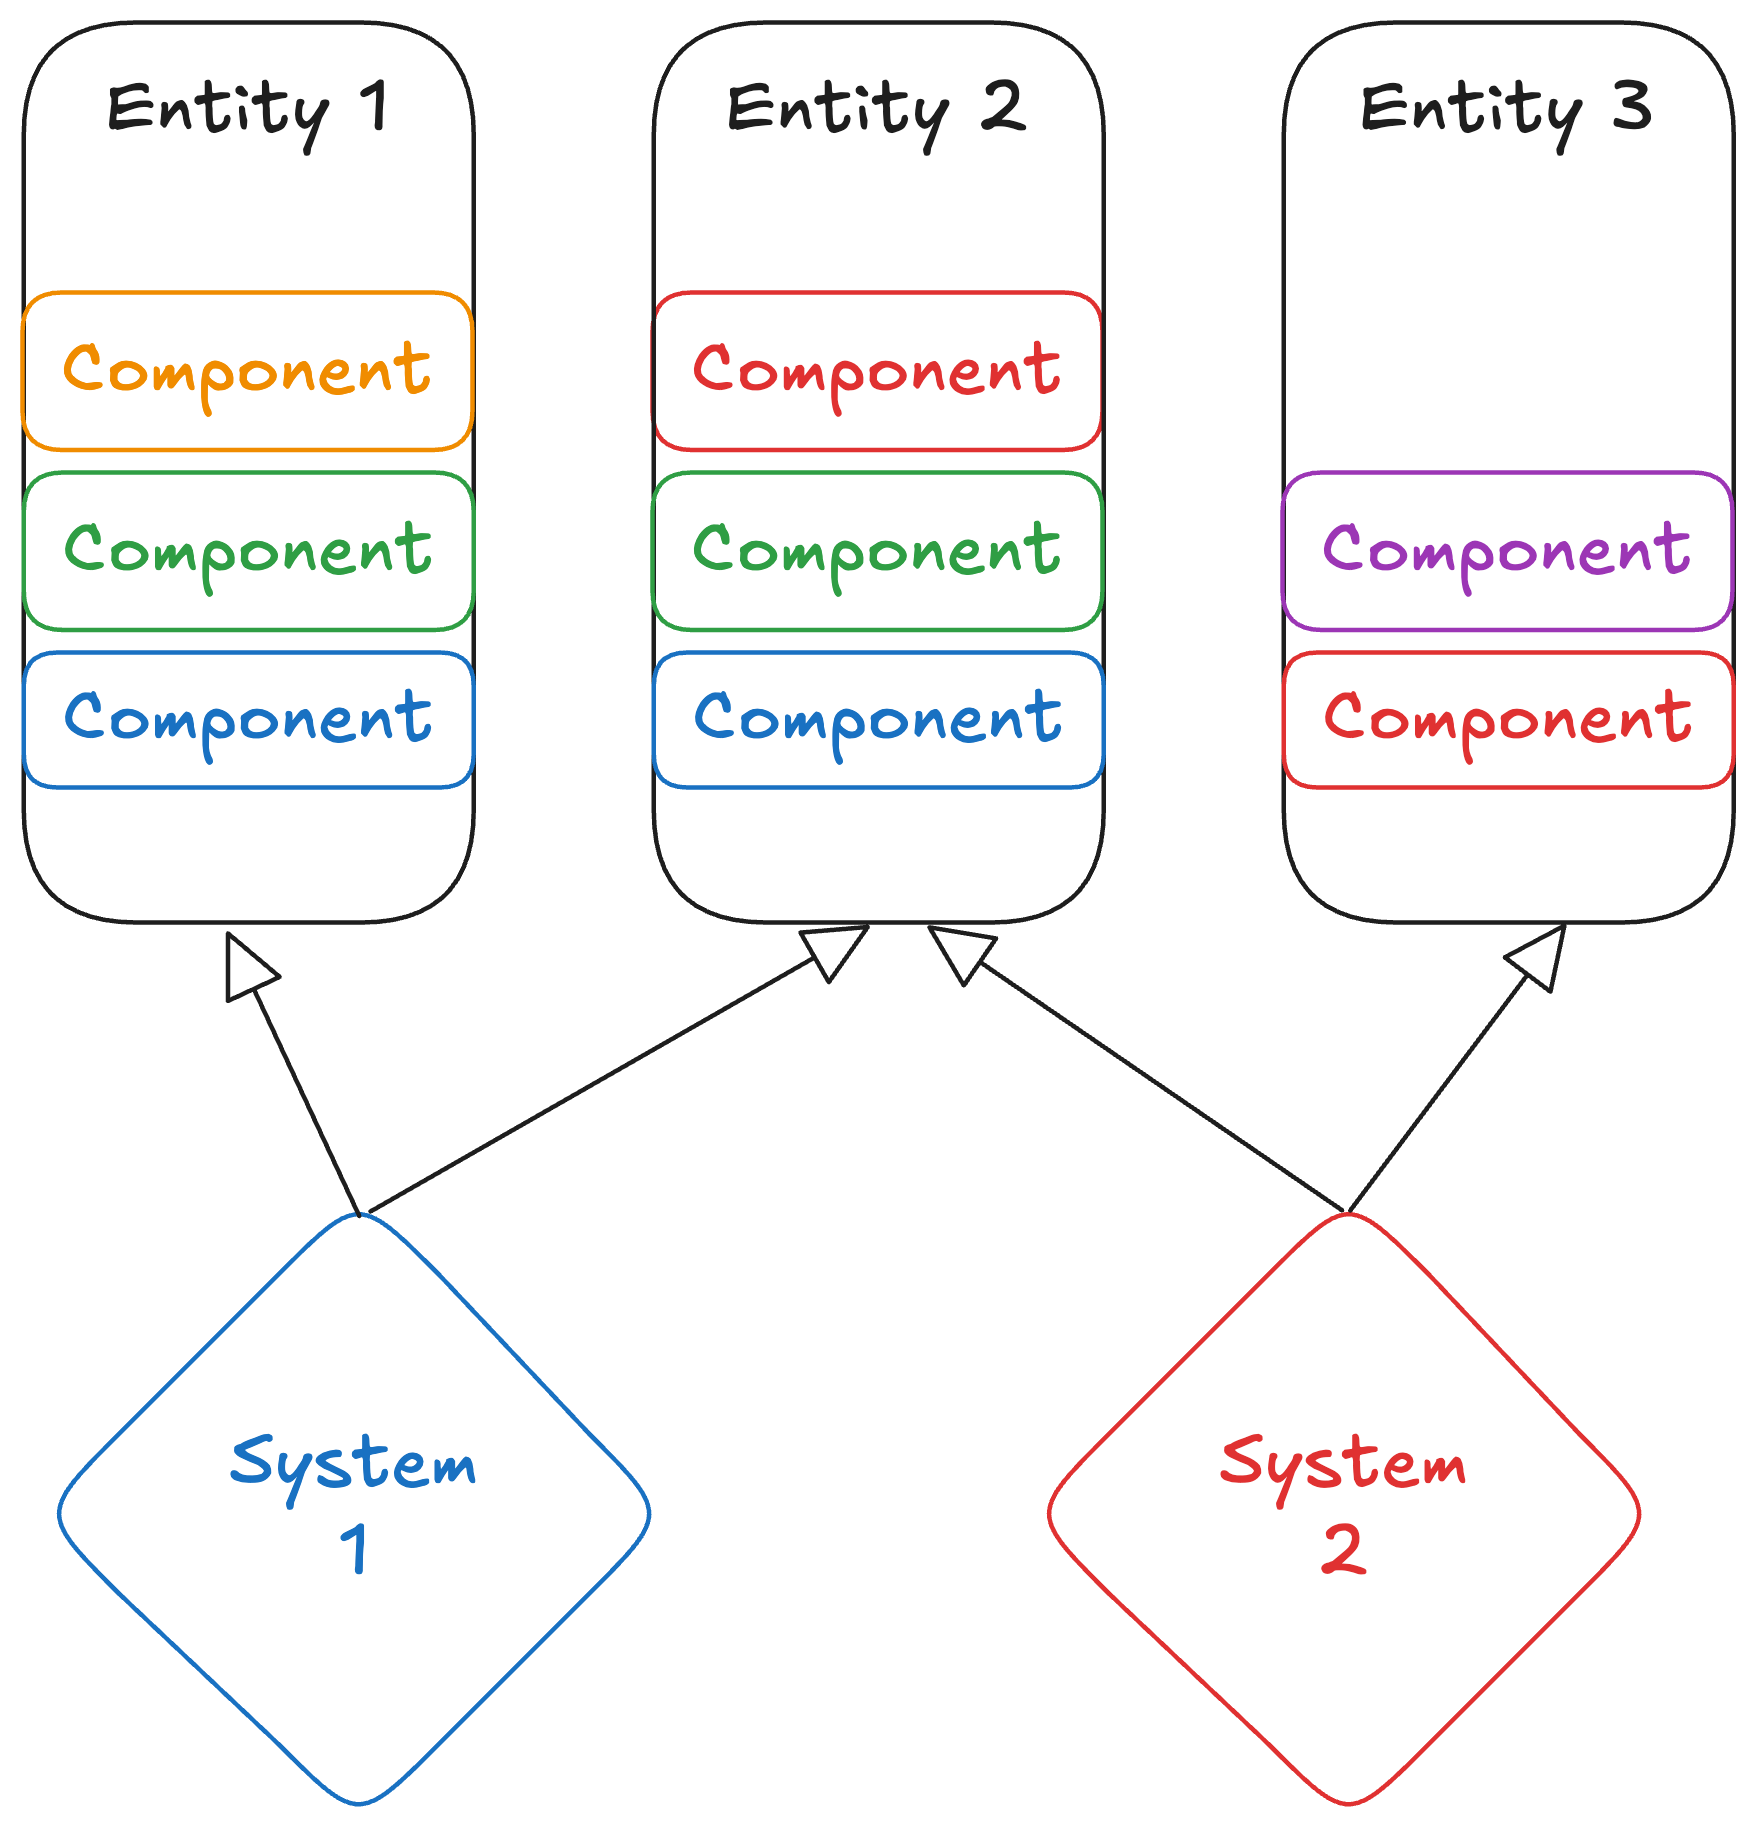
\includegraphics[width=0.2\linewidth]{assets/ECS-visualisatoin.png}
    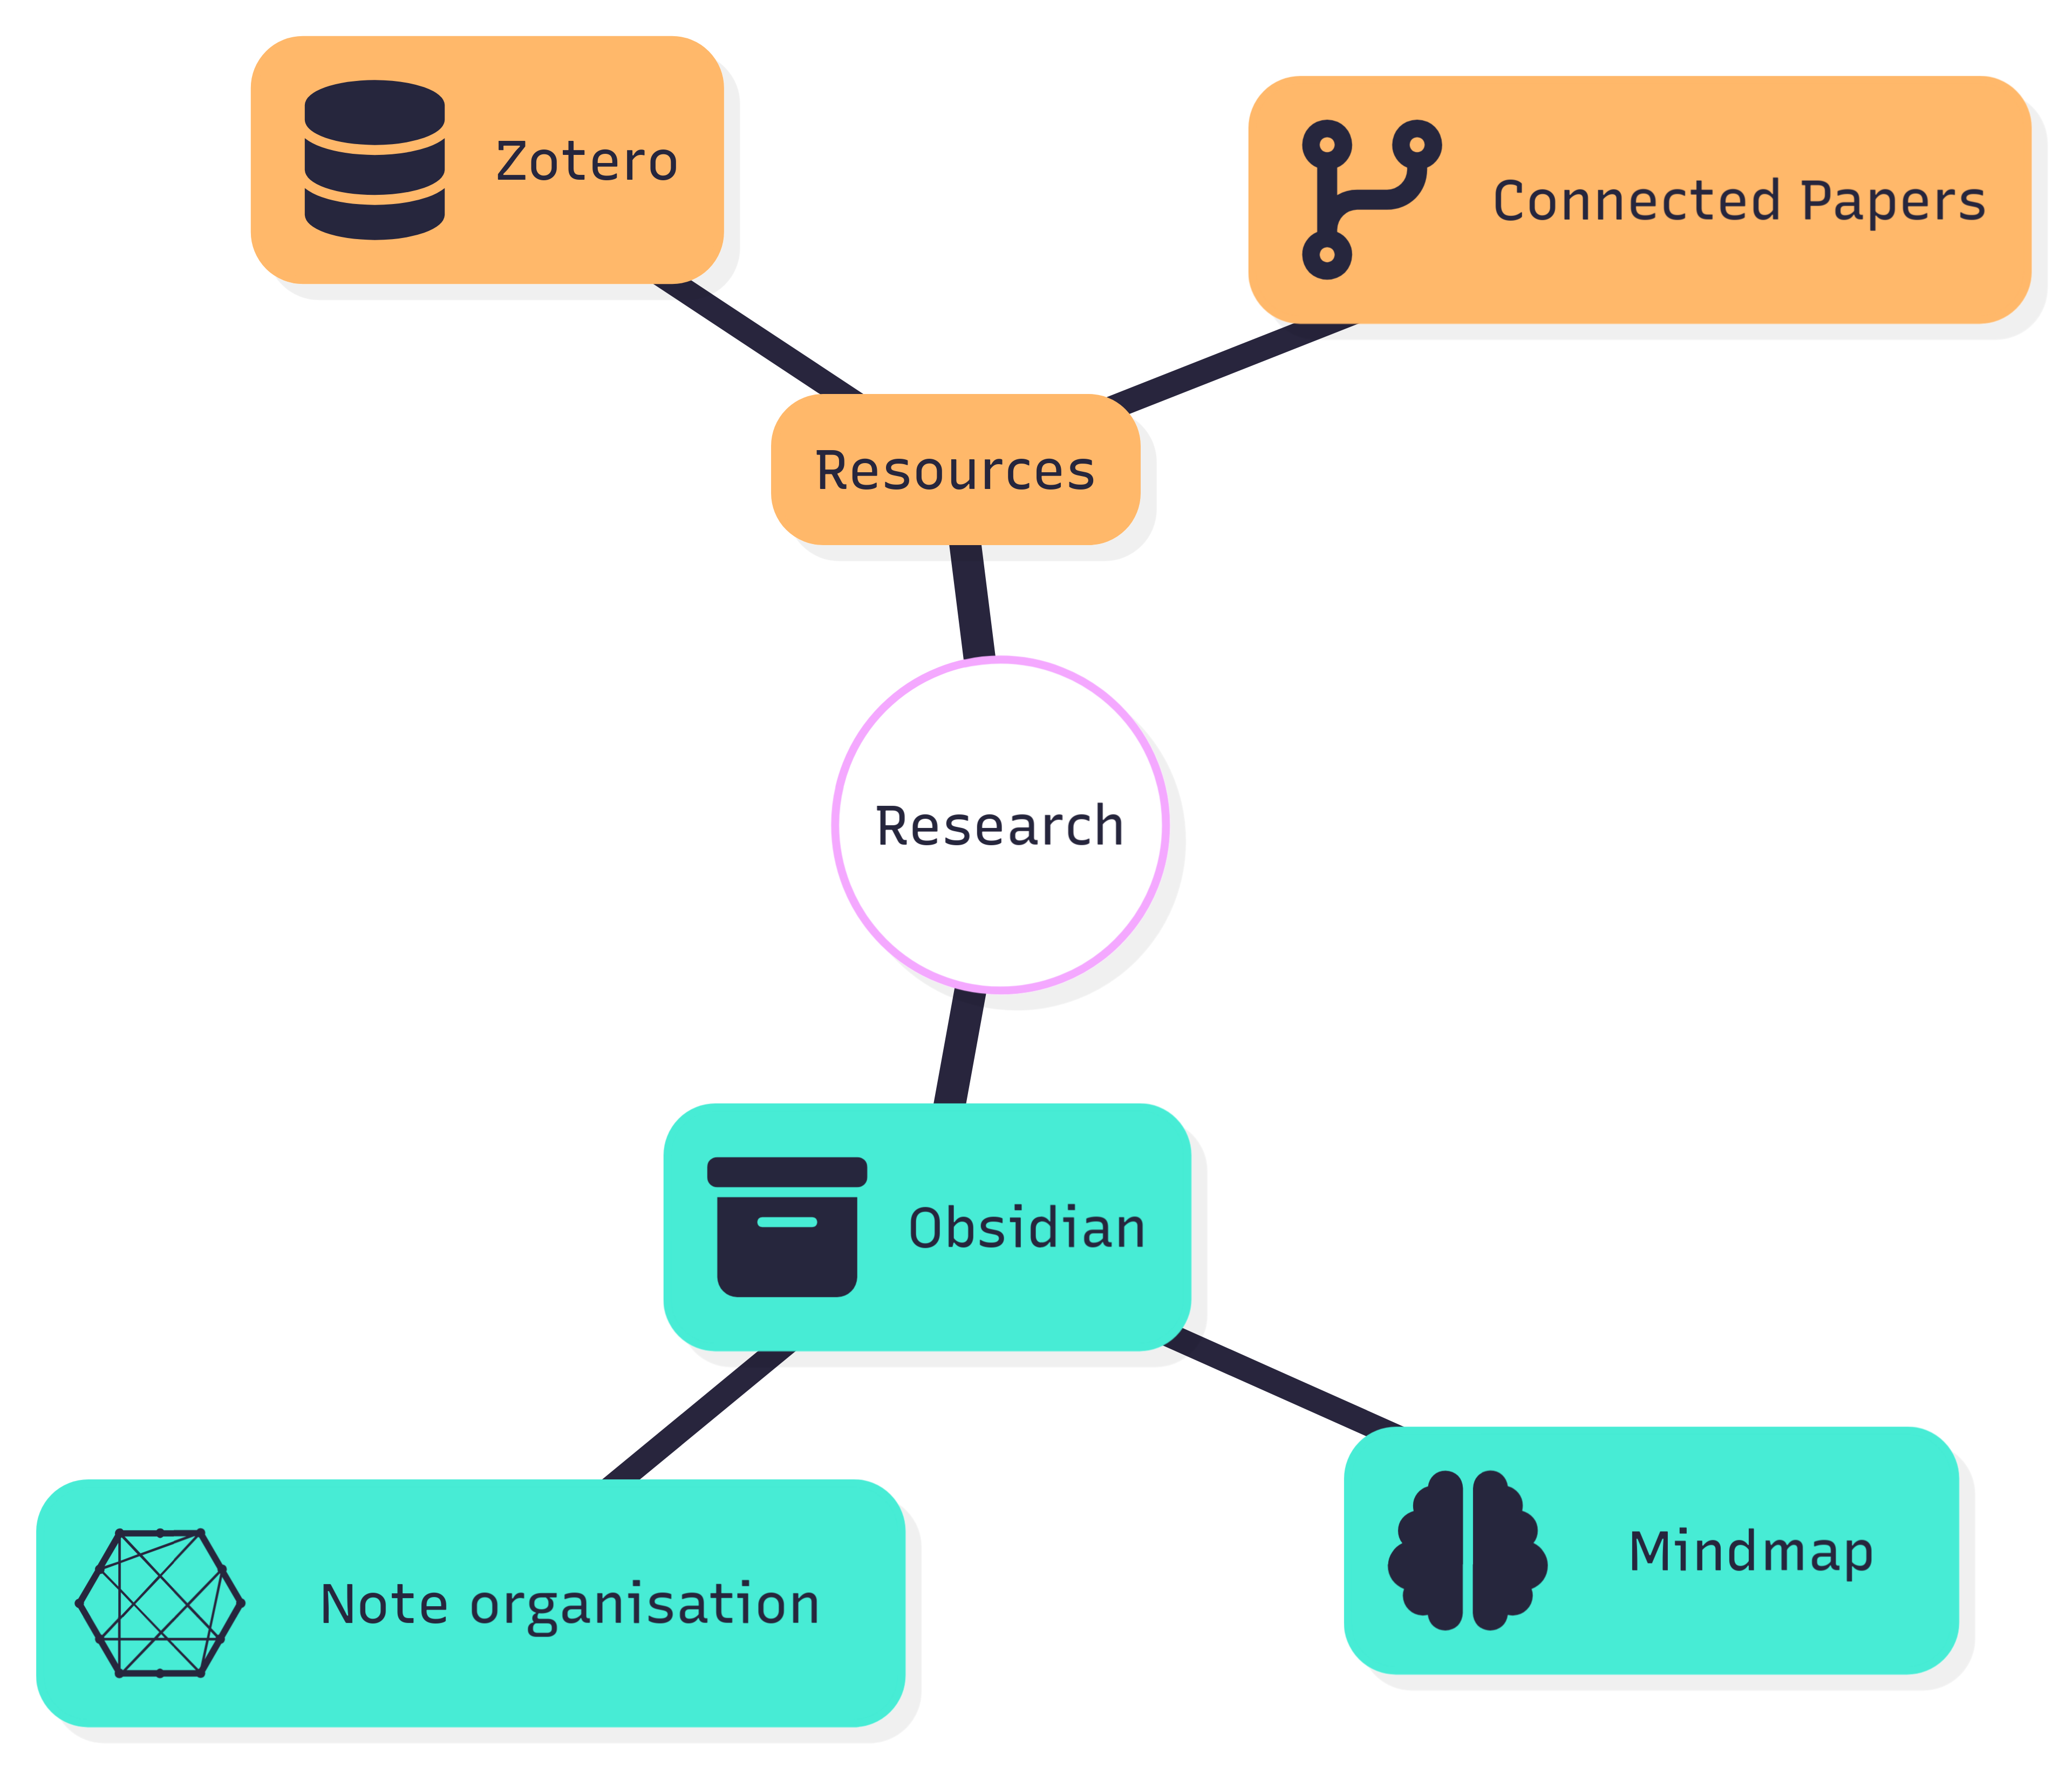
\includegraphics[width=0.2\textwidth]{assets/research-visualisation.png}
    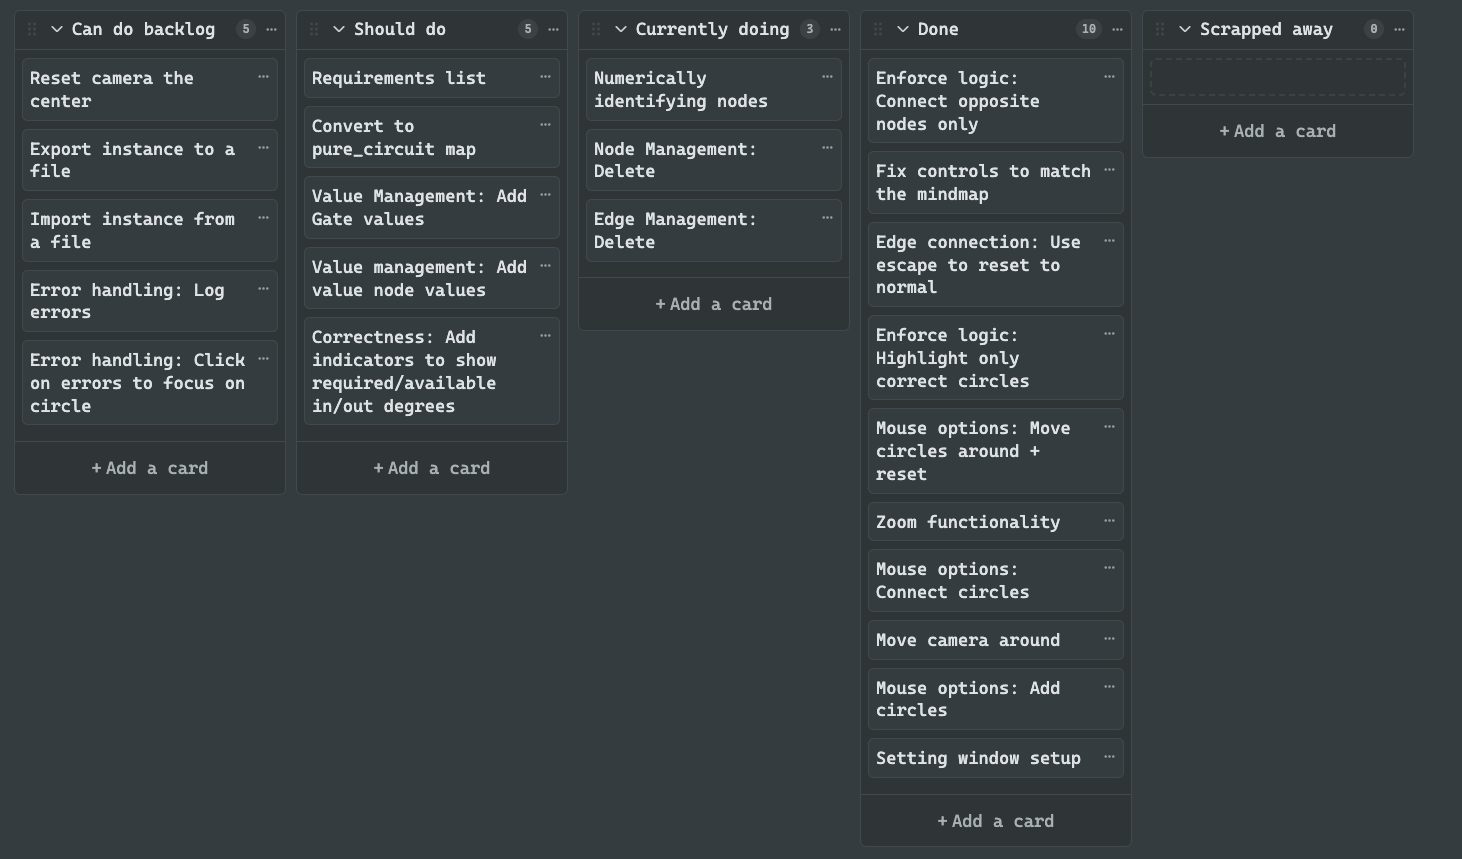
\includegraphics[width=0.2\textwidth]{assets/kanban-board.png}
    \caption{ECS workflow visualisation}
    \label{fig:soft:ecs-workflow}
\end{figure}

With regards to the our research management, we revolved our work around obsidian. As we can see in the figure \ref{fig:theory:obsidian-usages}, 
\texttt{Obsidian} beyond its traditional usage of note taking, it comes
with several handy tools such as note organisation and mind-mapping.



\begin{figure}[h!]
    \centering
    \subfloat[Obsidian Graph]{
        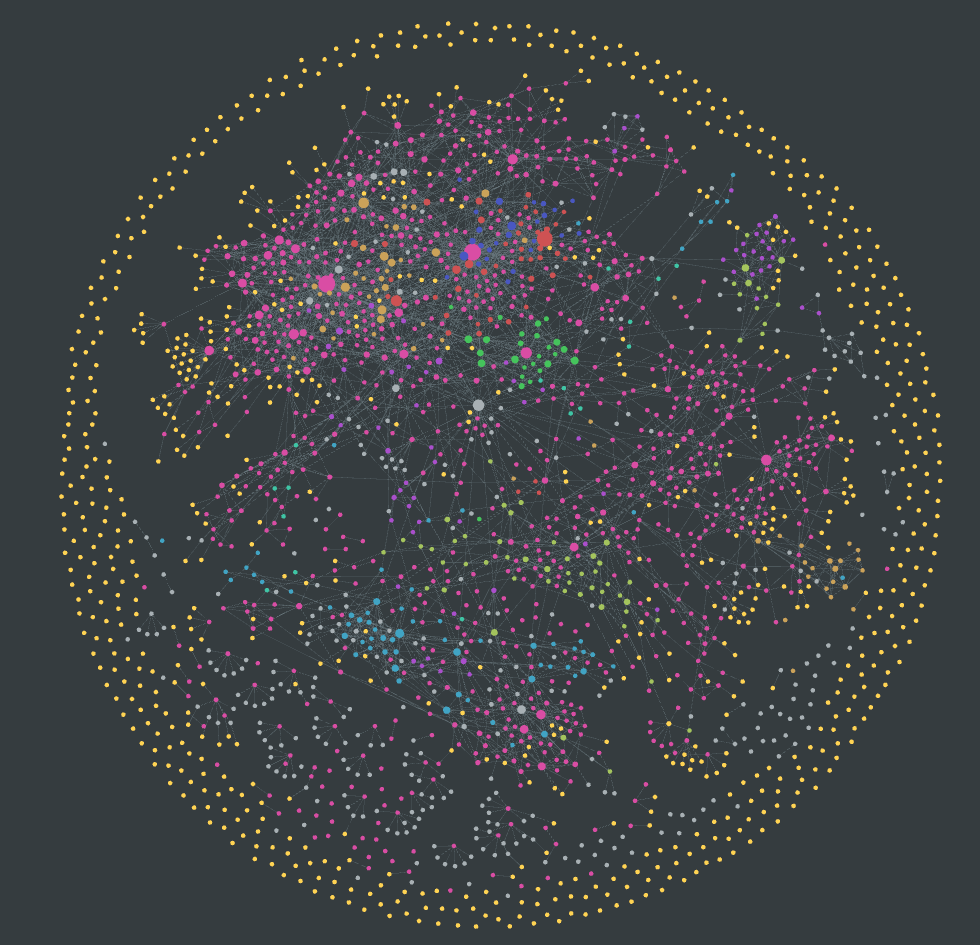
\includegraphics[width=0.3\linewidth]{assets/obsidian_graph.png}
        \label{fig:theory:obsidian-graph}
    }
    \subfloat[Obsidian Canvas]{
        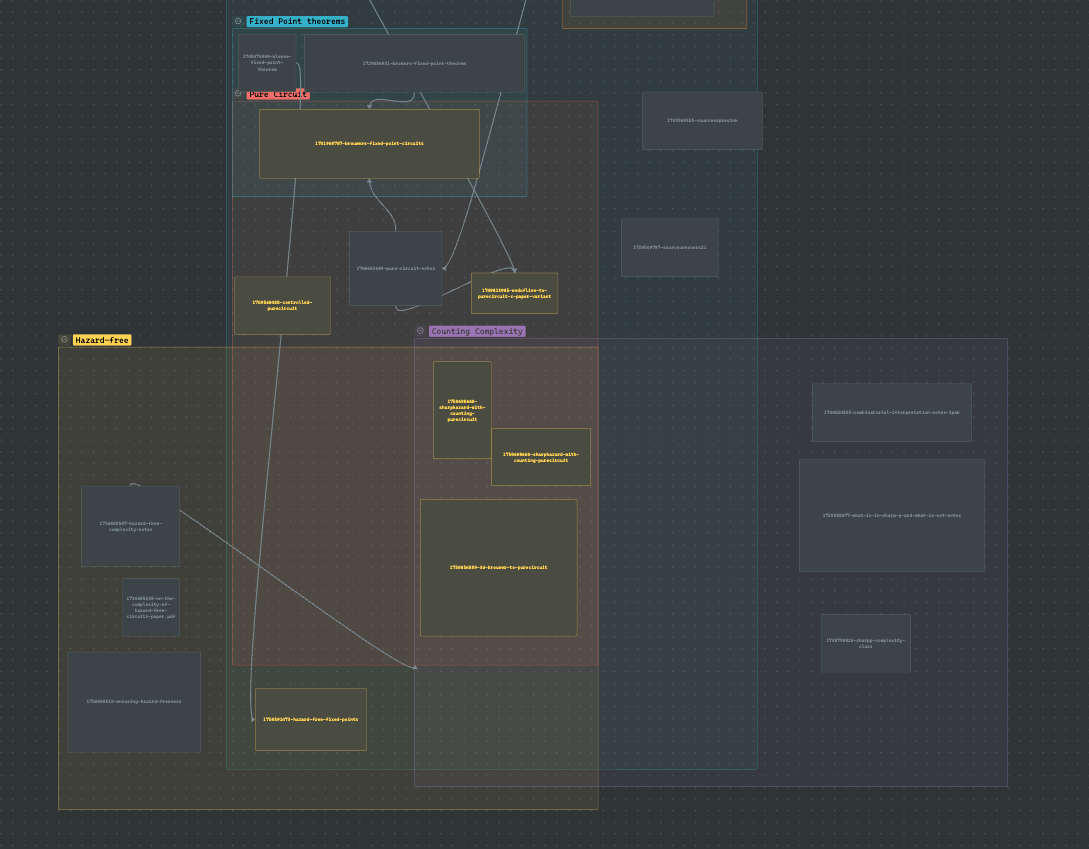
\includegraphics[width=0.3\linewidth]{assets/obsidian-canvas.png}
        \label{fig:theory:obsidian-canvas}
    }
    \subfloat[Obsidian mindmap]{
        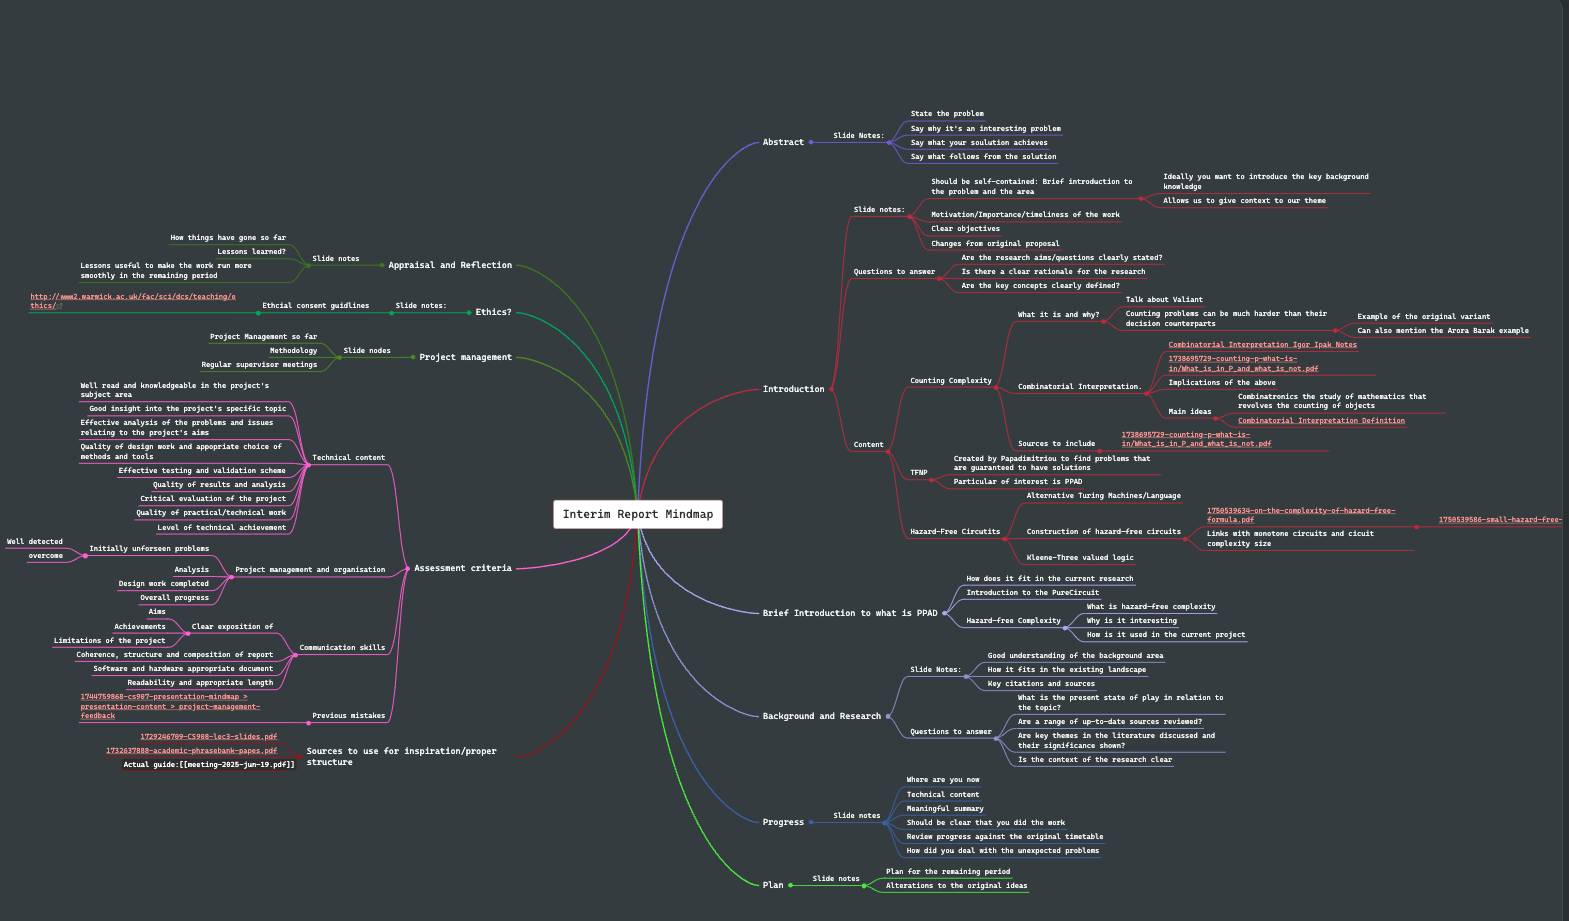
\includegraphics[width=0.3\linewidth]{assets/obsidian_mindmap.png}
        \label{fig:theory:obsidian-mindmap}
    }
    \caption{Usages of Obsidian}
    \label{fig:theory:obsidian-usages}
\end{figure}



\subsection{Risk Management}

With regards to risks and mitigations, the biggest risk we face
is the inability to resolve our main question. Due to the
limited literature surrounding \textsc{PureCircuit} and its
counting nature as well as the recency in the development of
$\textsc{TFNP} -1$, our question could go into many directions.
The discovery of our reduction allowed us to step closer to our question
and in our table \ref{tab:management:risk-management}, we will analyze this is greater depth.
The general mitigation strategy we can do is to keep researching, keep
finding connections until we can connect all the necessary pieces to do the jump.

\begin{xltabular}{0.95\linewidth}{|Z{1.2cm}|Z{1.75cm}|Y|Y|Z{1.2cm}|}
        \hline
        \textbf{Severity} & \textbf{Probability} & \textbf{Description} & \textbf{Mitigation} & \textbf{Address} \\
        \hhline{|=|=|=|=|=|}
        High   & Medium & Software may not be feasible within the remaining time frame. & Focus on the the first objective where the project. Restrict to solution finding or counting when the number of nodes is small. & Not yet      \\ \hline
        Low    & Medium & Software not identifying a correct solution & Usage of TDD techniques and property testing to ensure correctness.  Comparison with hand-made instances & Not yet      \\ \hline
        High   & High   & Inability to extend the reductions of the PureCircuit problem to SourceOrExcess & Find a path of parsimonious reductions between the two problems. If we cannot ensure a one-to-one relation between the solutions, we will focus on $1-c$ for some $c \in \mathbb{N}$  & $\checkmark$ \\ \hline
        Medium & High   & Inability to prove the main conjecture & We can make some heuristical arguments or find reductions between other problems. We argue that if we are able to unravel enough correlations, we will hope to at least bridge the problems. Develop useful gadgets one can use with PureCircuit & Not yet     \\ \hline
        High   & High   & Incorrect proofs or reductions. & Analyse the problem under different constraints. Apply the duck method, where attempt to explain the solution to a person which not necesserily an expert. Validate proof with supervisor & Not yet  \\ \hline
        High   & Medium & Develop combinatorial friendly variants of \textsc{PureCircuit} & Apply robustness on the gate set of \textsc{PureCircuit}. Develop new gates or variants are easier to work with.  & $\checkmark$  \\ \hline
        \caption{Risk managment table.} \label{tab:management:risk-management}
\end{xltabular}


From our table, it is worth expanding on some of the points. The best method
we found when tackling this problem is when we try to uncover reductions between other
PPAD problems or when trying to incorporate gadgets from Kleene theory. We hope
that by expereminting enough we will be able to get close to resolve our conjectures.

